\section{Module 3. Non-stationary noise estimation}
In order to test effectiveness of implemented algorithm the results of it were compared to results of algorithm prepared to perforem calculatioans contained in \cite{aja2015spatially} (the algorithm for the article was implemented in Matlab). The comparison of these the two kinds maps was based on the result of subtracting Python map from Matlab. It was done for four maps estimated for corrupted MRI images.
\begin{itemize}
\item \textbf{Image 1}
\begin{figure}[H]
	\centering
	\captionsetup{justification=centering}
		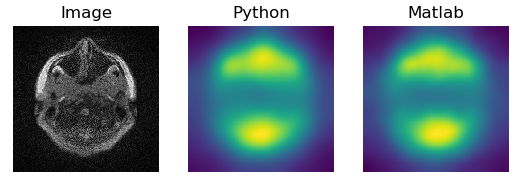
\includegraphics[scale=0.7]{figures/module03/10_comp}
		\caption{Image (left), noise map form Python algorithm(middle), noise map form Matlab algorithm(right).}
\end{figure}
\begin{table}[H]
\caption{\label{tab:table-name}Parameters calculated for image 1.}
	\begin{center}
		\begin{tabular}{ |c|c|c|c|c|c| } 
 			\hline
 			\textbf{Python map mean} & \textbf{Matlab map mean} & \textbf{Difference mean} & \textbf{Difference SD} & \textbf{Max. difference} & 					\textbf{Min. difference} \\ 
			\hline
 			11.8741 & 11.3964 & -0.4776 & 0.7485 & 1.6136 & -2.7325 \\ 
			\hline
		\end{tabular}
	\end{center}
\end{table}
\item \textbf{Image 2}
\begin{figure}[H]
	\centering
	\captionsetup{justification=centering}
		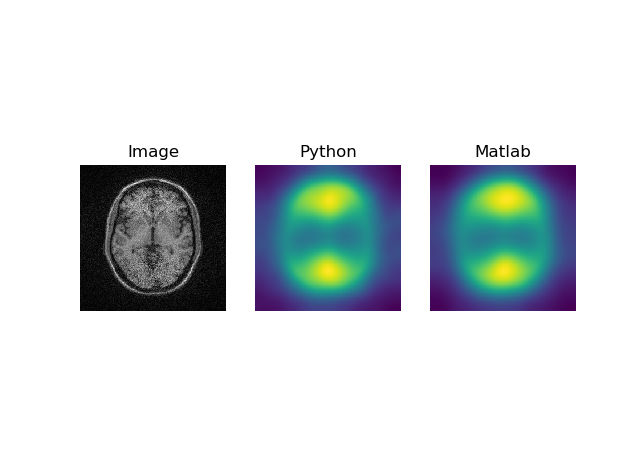
\includegraphics[scale=0.7]{figures/module03/70_comp}
		\caption{Image (left), noise map form Python algorithm(middle), noise map form Matlab algorithm(right).} 
\end{figure}
\begin{table}[H]
\caption{\label{tab:table-name}Parameters calculated for image 2.}
	\begin{center}
		\begin{tabular}{ |c|c|c|c|c|c| } 
 			\hline
 			\textbf{Python map mean} & \textbf{Matlab map mean} & \textbf{Difference mean} & \textbf{Difference SD} & \textbf{Max. difference} & 					\textbf{Min. difference} \\ 
			\hline
 			12.5484 & 11.8232 & -0.7253 & 0.8646 & 0.9555 & -2.9163 \\ 
			\hline
		\end{tabular}
	\end{center}
\end{table}
\item \textbf{Image 3}
\begin{figure}[H]
	\centering
	\captionsetup{justification=centering}
		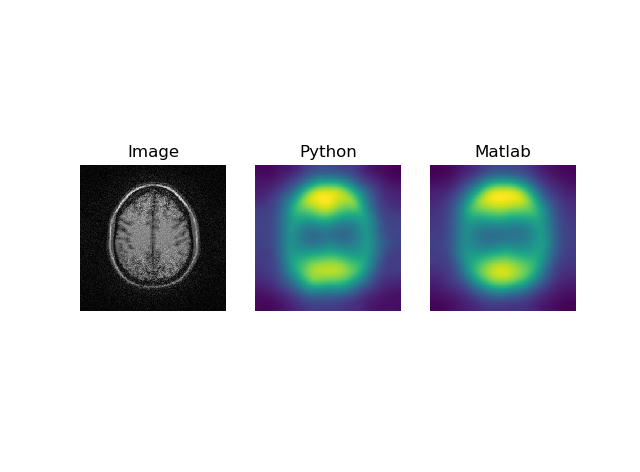
\includegraphics[scale=0.7]{figures/module03/110_comp}
		\caption{Image (left), noise map form Python algorithm(middle), noise map form Matlab algorithm(right).} 
\end{figure}
\begin{table}[H]
\caption{\label{tab:table-name}Parameters calculated for image 3.}
	\begin{center}
		\begin{tabular}{ |c|c|c|c|c|c| } 
 			\hline
 			\textbf{Python map mean} & \textbf{Matlab map mean} & \textbf{Difference mean} & \textbf{Difference SD} & \textbf{Max. difference} & 					\textbf{Min. difference} \\ 
			\hline
 			12.1854 & 11.4882 & -0.6972 & 0.9245 & 0.8657 & -3.3731 \\ 
			\hline
		\end{tabular}
	\end{center}
\end{table}
\item \textbf{Image 4}
\begin{figure}[H]
	\centering
	\captionsetup{justification=centering}
		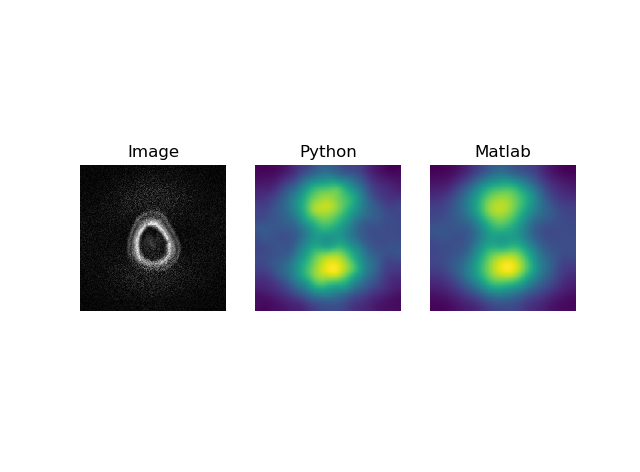
\includegraphics[scale=0.7]{figures/module03/160_comp}
		\caption{Image (left), noise map form Python algorithm(middle), noise map form Matlab algorithm(right).} 
\end{figure}
\begin{table}[H]
\caption{\label{tab:table-name}Parameters calculated for image 4.}
	\begin{center}
		\begin{tabular}{ |c|c|c|c|c|c| } 
 			\hline
 			\textbf{Python map mean} & \textbf{Matlab map mean} & \textbf{Difference mean} & \textbf{Difference SD} & \textbf{Max. difference} & 					\textbf{Min. difference} \\ 
			\hline
 			10.2958 & 10.3830 & 0.0873 & 0.5942 & 1.1861 & -2.1734 \\ 
			\hline
		\end{tabular}
	\end{center}
\end{table}
\end{itemize}
Results from Python algorithm are not perfect equivalent of the results from Matlab algorithm, however they are very similar and seem to be suitable for 
further processing of the image.
\begin{table}[H]
\small
\caption{\label{tab:table-name}Juxtaposition of parameters calculated all images.}
	\begin{center}
		\begin{tabular}{ |c|c|c|c|c|c|c| } 
 			\hline
 			 & \textbf{Python map mean} & \textbf{Matlab map mean} & \textbf{Difference mean} & \textbf{Difference SD} & \textbf{Max. difference} & 				\textbf{Min. difference} \\ 
			\hline
 			\textbf{1} & 11.8741 & 11.3964 & -0.4776 & 0.7485 & 1.6136 & -2.7325 \\ 
			\hline
			\textbf{2} & 12.5484 & 11.8232 & -0.7253 & 0.8646 & 0.9555 & -2.9163 \\ 
			\hline
			\textbf{3} & 12.1854 & 11.4882 & -0.6972 & 0.9245 & 0.8657 & -3.3731 \\ 
			\hline
			\textbf{4} & 10.2958 & 10.3830 & 0.0873 & 0.5942 & 1.1861 & -2.1734 \\ 
			\hline
			\textbf{Mean} & 11.7259 & 11.2727 & -0.4532 & 0.7829 & 1.1552 & -2.7988 \\ 
			\hline
		\end{tabular}
	\end{center}
\end{table}